\documentclass[crop, tikz]{standalone}

\usepackage{tikz}
\usetikzlibrary{matrix,positioning}
\begin{document}
	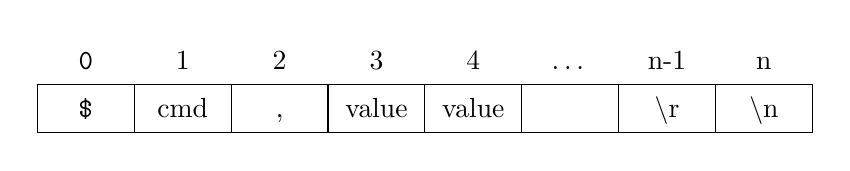
\begin{tikzpicture}[cell/.style={rectangle,draw=black},
	space/.style={minimum height=1.5em,matrix of nodes,row sep=-\pgflinewidth,column sep=-\pgflinewidth,column 1/.style={font=\ttfamily}},text depth=0.5ex,text height=2ex,nodes in empty cells]
	

	
	\matrix (first)[space, row 2/.style={minimum width=3em,nodes={cell,minimum width=3.5em}},row 3/.style={nodes={cell,minimum width=2em}}]
	{
		0   & 1  & 2 & 3 & 4& \ldots & n-1&n  \\   
		\$  & cmd  & , & value & value &  & \textbackslash r &  \textbackslash n \\};
	
	
	
	
	\end{tikzpicture}
\end{document}